\documentclass[a4paper]{article}
\usepackage{geometry}
\usepackage{authblk}
\usepackage{listings}
\usepackage{array}
\usepackage{amsmath}
\usepackage{amssymb}
\usepackage{amsfonts}
\usepackage{amscd}
\usepackage{tikz}
\usetikzlibrary{snakes,arrows,shapes}
\usepackage{graphicx}
%\usepackage{caption}
\usepackage{appendix}
\usepackage{hyperref}
\usepackage[utf8]{inputenc}
\usepackage[round]{natbib}
\usepackage{bm}
%\usepackage{chemist}
%\usepackage{chemformula}
\usepackage{breqn}
\usepackage{enumitem}
\usepackage{setspace} %needed for preprint in doublelinespace 
%\usepackage[colorinlistoftodos, textwidth=4cm, shadow]{todonotes} %comments and
\usepackage[normalem]{ulem} % provides strike out
\usepackage{caption}
\DeclareRobustCommand{\figref}[1]{ Fig. \ref{#1}}
\DeclareRobustCommand{\revref}[1]{Comment: \ref{#1}}
\DeclareRobustCommand{\Theoref}[1]{Theorem \ref{#1}}
\DeclareRobustCommand{\Defref}[1]{\mbox{Definition \ref{#1}}}
\DeclareRobustCommand{\enumref}[1]{\ref{#1}}
\DeclareRobustCommand{\appendixref}[1]{appendix \ref{#1}}
\DeclareRobustCommand{\Appendixref}[1]{Appendix \ref{#1}}
\DeclareRobustCommand{\sectionref}[1]{ section \ref{#1}}
\DeclareRobustCommand{\tupelref}[2]{\enumref{#1} \enumref{#2}}
%\definecolor{dark-green}{rgb}{0,0.25,0}
% vectors and matrices
\renewcommand{\vec}[1]{\boldsymbol{\mathbf{#1}}}
\newcommand{\tens}[1]{\mathrm{#1}}

% d/dt not italic, dt in integrals d upright, even putting the space before
\newcommand{\deriv}[1]{\frac{\mathrm{d}}{\mathrm{d}#1}}
\newcommand{\dd}[1]{\,\mathrm{d}#1}
\newcommand{\pderiv}[1]{\frac{\partial}{\partial #1}}

\newcommand{\suml}{\sum\limits}
\newcommand{\prodl}{\prod\limits}
\newcommand{\intl}{\int\limits}
\newcommand{\liml}{\lim\limits}
\newcommand{\LAPM}{\texttt{LAPM}}
\newcommand{\CompartmentalSystems}{\texttt{CompartmentalSystems}}
\newcommand{\ComputabilityGraphs}{\texttt{ComputabilityGraphs}}
%\newcommand{\bgc_md2}{\texttt{bgc \textunderscore md2}}

% numbers
\newcommand{\N}{numbersystem:N}
\newcommand{\R}{numbersystem:R}
\newcommand{\CN}{numbersystem:C}
\newcommand{\Rpd}{numbersystem:Rpd}
\newcommand{\Rp}{numbersystem:Rp}

\newcommand{\tnot}{\gls{symb:t0}}
\newcommand{\transpose}{symb:transpose}


\title{The biogeochemichal model data base \texttt{bgc\_md2} and python
packages  \LAPM, \CompartmentalSystems, \ComputabilityGraphs for the analysis of compartmental dynamical systems}
\date{\today}
\author[1]{M{arkus M{\"{u}}ller}}
\author[1]{Holger Metzler}
\author[1]{Ver{\'{o}}nika Ceballos-N{\'{u}}{\~{n}}ez}
\author[1]{Carlos A. Sierra}
\affil[1]{Max Planck Institute for Biogeochemistry, Hans-Knöll-Str. 10, 07745 Jena, Germany}

\begin{document}
\maketitle

\begin{abstract} \noindent
Compartmental systems are a particular class of dynamical systems that describe
  the flow of conserved quantities such as mass and energy through a network of
  interconnected compartments. 
  The main purpose and greatest challenge of this work is to make such models
  {\bf transparent} by  facilitating  comparisons between them.
  To this end we enhance the common diagnostics of pool contents and fluxes by the
  implementing the computations of age and
  transit time distributions for all models.
  We create a language to describe different models in different ways with
  respect to common eqivalent building blocks, and start and extendable
  collection of models.
  We can compare not only what is formulated in the model description but what is 
  {\bf computable}. 
  To this end we  developed three python packages for the
  mathematical analysis and computation of system-level metrics for distinct
  groups of compartmental systems. 
  \LAPM (Linear Autonomous Pool Models)
  provides functions for the analysis of compartmental systems at
  equilibrium. 
  \CompartmentalSystems tools for the
  analysis of non-autonomous linear compartmental systems. 
  To study properties of groups of models and make comparisons among them, we developed
  the package \texttt{bgc\_md2} (Biogeochemical Model Database ), motivated by our own work
  on the terrestrial carbon cycle.
  \ComputabilityGraphs can determine the set of all possible computations that
  can be performed on a model depending on information available from its
  description, allowing to query \texttt{bgc\_md2}'s collection of models.
  The implemented analysis tools include symbolic computations  
  of model decomposition into subsystems, flowdiagrams, transformation and reformulation with respect to
  different building blocks e.g. matrix versus flux equations and also 
  difficult to obtain numerical metrics to characterize timescales
  of mass flow in compartmental systems such as the age of the mass and transit time
  trough the entire system, subsystems like vegetation or soil, or individual
  compartments.
  Together, these packages offer advanced integrated 
  tools for the symbolic and numerical characterization of
  compartmental dynamical systems.
\end{abstract}

\section{Motivation and significance}
The principle of mass conservation plays a central role in mathematical models
of natural systems in a variety of scientific fields such as systems biology,
toxicology, pharmacokinetics \citep{Anderson1983}, ecology
\citep{Eriksson1971ARoEaS, Rodhe1979Tellus, Matis1979, Manzoni2009SBB},
hydrology \citep{Nash1957IASH, Botter2011GRL, Harman2014GRL}, biogeochemistry
\citep{Manzoni2009SBB, Sierra2015EM}, and epidemiology \citep{Jacquez1993SIAM}.
In most cases such models are nonnegative dynamical systems that can be
described by first-order systems of ordinary differential equations (ODEs) with
strong structural constraints.  Such systems are called compartmental systems
\citep{Anderson1983, Jacquez1993SIAM, Walter1999, Haddad2010}, and have
important mathematical properties that aid in their analysis and study.

As mass moves across a compartmental system, it is often of interest to study
properties of the compartments, the entire system or subsystems related to the speed at
which the mass moves, and the time it takes mass to pass through specific
paths. These properties are generally characterized
by metrics such as the age of mass with respect to the entry to the entire
system, a subsystem, or a single compartment and the transit time of mass 
across the entire network of compartments or parts of it until its
final exit. 
However, there are different methods to compute these metrics from
compartmental systems depending on specific assumptions imposed on the system
of equations \citep{Sierra2017GCB}. and available computational
procedures may differ largely depending on specific assumptions.

To aid in the analysis of compartmental systems, and to determine the type of
computational methods that can be performed for particular systems under given
assumptions, we developed four python packages for their representation,
classification, and analysis. These open source packages are called: 
\LAPM (Linear Autonomous Pool Models),
\CompartmentalSystems, 
\texttt{bgc\_md2} (Biogeochemical Model Database), and
\texttt{ComputabilityGraphs}.

This manuscript provides a general introduction to these four python packages,
with emphasis of their combined use via \texttt{bgc\_md2} ,
and aims at providing a general guidance for their use, installation, and
modification. 
We provide an example based on the global carbon cycle, but the
packages can be used for a large variety of systems in which mass or energy
conservation is required.

%:
\section{Conceptual framework}
\subsection{Definition and classification of compartmental systems}
Compartmental systems describe the dynamics of a vector fo mass contents $x$ of $n$ kinetically homogeneous compartments. Because mass is a non-negative quantity, this vector of mass contents can only occupy the non-negative orthant of the state-space; i.e. $x \in \mathbb{R}^n_+$. A compartmental system generally receives mass from outside the system according to a vector of mass inputs $u \in \mathbb{R}^n_+$, and this mass is transferred among compartments and released back to the external environment according to rates encoded in a compartmental matrix $B \in \mathbb{R}^{n \times n}$. Therefore, we can write the dynamics of a compartmental system as a set of ordinary differential equations of the form
\begin{equation} \label{eq:CompartmentalSystem}
\frac{dx}{dt} = \dot{x} = u(x, t) + B(x, t) \, x(t)
\end{equation}
The key property of compartmental systems is, in order for the system to balance mass, that the square matrix $B=(B_{ij})$ exhibits three main properties
\begin{enumerate}
  \item $B_{ii}\leq0\text{ for all }i$,
  \item $B_{ij}\geq0\text{ for all }i\neq j$, and
  \item $\suml_i B_{ij}\leq 0\text{ for all }j$.
\end{enumerate}
Then, $\tens{B}$ is called \emph{compartmental} and governs all internal cycling of material as well as the exit of material from the system.

We distinguish between different types of compartmental systems, according to linearity and autonomy. If the vector of inputs and the compartmental matrix depend on the vector of states in system \eqref{eq:CompartmentalSystem}, we call it non-linear, and linear otherwise. Similarly, if the vector of inputs and the compartmental matrix depend on time, we call the system non-autonomous, and autonomous otherwise. 

\subsection{System level metrics: age, transit time, and entropy}
Compartmental systems can be described by a set of metrics that characterize system level properties. 
Ages, transit times, and entropies are key quantities of compartmental systems that can be considered to better understand underlying system dynamics and to compare models with different sizes or structures.
While age describes how old material in the system is, transit time describes how long material needs to travel through the entire system from entry to exit \citep{bolin1973Tellus, Sierra2017GCB}.
These quantities provide us with information about the timescales at which systems operate and respond to perturbations.

The Shannon information entropy can be used as a complexity measure  to characterize the complexity of dynamical systems \citep{Ebeling1998}.
It can be used to describe the uncertainty of a particle's path through a compartmental system, quantifying how difficult it is to predict this path. It can be used for comparing path properties of models with different number of compartments and connections among them \citep{Metzler2020}.

\subsection{Compartmental systems in equilibrium} \label{sec:Equilibrium}
The concept of equilibrium is restricted to autonomous systems. It does not even make sense to ask the question otherwies. 
If the autonomous system is nonlinear it is possible but not certain that an
equilibrium exists. The only case where we can expect an equilibrium are
linear, autonomous, pool models, 
\begin{equation} \label{eq:LS}
\dot{x} = u + B \, x, \qquad  \mathrm{with} \quad x(t_0) = x_0.
\end{equation}
for which interesting properties can be
obtained by the \LAPM package.  The equilibrium $x^*$ is defined by the
condition  $\dot{x^*}=0$ which translates to $-B x*=u$ which means that for
pool contents $x*$ the influxes $u$ match the outfluxes $B x*$ exactly.  It is
straightforward to see that for this to happen all 
pools with influxes must be connected (possibly via other pools) to an outflux of
the system, and that the (constant) rates for all the flux rates out of all
pools along this paths are greater than zero, since an input receiving pool $p$
without these conditions would necessarily grow over time, violation the
equilibrium condition $\dot{x*}_p=0$. Interestingly these conditions also
gurantee that $B$ is invertable and the equilibrium therefore uniquely
determined by: 
\begin{equation} 
x^* = - {B^*}^{-1} \, u^*.  
\end{equation}
Although at different times different material moves through the system, the
size of the pools does not depend on time if the system is in
equilibrium: $x(t)=x^*$ 
This is also true for other properties such as the
age distribution of mass in particular compartments and in the entire system
and the transit time distribution, which is defined as the time it take masses
in the input flux to appear in the output flux.  Although the material moving
through the system does change the amount, age and transit
time distributions do not.  They are in fact characterized by the Phase Type
distribution, which depends on compartmental matrix $B$ and the equilibrium
solution $x^*$ for the system age distribution and the $B$ and the input $u$
for the transit time distribution \citep{Metzler2018MGS}.
Compartmental systems at equilibrium have similar properties as continuous-time absorbing Markov Chains \citep{Metzler2018MGS}. Therefore, we can obtain other quantities of interest such as  the path entropy of particles that travel across the system and the occupation time of particles inside compartments \citep{Metzler2020}. These properties of linear autonomous compartmental systems at equilibrium can be obtained with the \LAPM package.

Interestingly the properties of linear autonomous systems in equilibrium can
also be computed for nonlinear systems in equilibrium if such an equilibrium
exists.
\begin{equation} \label{eq:NLS}
\dot{x} = u(x) + B(x) \, x, \qquad  \mathrm{with} \quad x(t_0) = x_0,
\end{equation}
In equilibrium the system is indistinguishable from a linear autonomous one
\begin{align} 
  0= \dot{x^*} = u^* + B^* \, x^*
\end{align}
with $B^*=B(x^*)$ and $u^*=u(x^*)$ 
Therefore also  nonlinear autonomous
systems at equilbrium can be analyzed with the by the
\LAPM package.
Note however,that we no such $x^*$ might not exist for some systems
while others may have multiple equilibrium solutions and the age and
transittime distribution may be very different for these different equilibria.

%%%%%%%%%%%%%%%%%%%%%%%%%%%%%%%%%%%%%%%%%%%%%%%%%%%%%%%%%%%%%%%%%%%%%%%%%%%%
\subsection{Time evolution along a trajectory} \label{sec:trajectory}
We consider now linear non-autonomous systems of the form
\begin{equation} \label{eq:NALS}
\dot{x}(t) = u(t) + B(t) \, x, \qquad  \mathrm{with} \quad x(t_0) = x_0.
\end{equation}
In this case, the inputs and the compartmental matrix are time-dependent and
the system never converges to a fixed-point solution. In most cases, an
analytical solution cannot be obtained, but the solution can be 
obtained numerically. In particular, the solution for systems of the form of equation \eqref{eq:NALS} can be written as
\begin{equation}
x(t, t_0, x_0) = \Phi(t, t_0) x_0 + \int_{t_0}^{t} \Phi(t, \tau) u(\tau) \mathrm{d}\tau.
\end{equation}
The state transition operator $\Phi(t,t_0)$ is a matrix-valued function that
multiplied with the state $x_0$ at $t_0$ transitions it to the state $x(t)$
subsequent time $t > t_0$. It is numerically computable by solving an matrix
ode derived from \eqref{sec:trajectory} 
From $\Phi(t,t_0)$ we can obtain not only the temporal evolution of the
solution $x(t)$ but also of the distributions of ages of the mass in the compartments and in the entire system \citep{Metzler2018PNAS}.
The \CompartmentalSystems package provides all the functionality necessary to do these computations, which rely on a description of the time-dependent input vector $u(t)$ and the compartmental matrix $B(t)$, as well as initial age distributions for the compartments.

Furthermore, these computations can also be obtained for nonlinear systems of the form
\begin{equation} \label{eq:NANLS}
\dot{x}(t) = u(t, x) + B(t, x) \, x(t), \qquad  \mathrm{with} \quad x(t_0) = x_0.
\end{equation}
by numerically solving \eqref{eq:NANLS} and plugging the solution $x(t, t_0,
x_0)$ back into it, which results in $\tilde{B}(t)=B(t,x(t, t_0,x_0))$ and
$\tilde{u}(t)=u(t,x(t, t_0,x_0)$  i.e a linear system in the form
\eqref{eq:NALS}. 
Therefore,  age and transit time
distributions can be obtained for nonlinear non-autonomous systems along the
specific trajectory. Detailed methods for the computation are provided in
\citet{Metzler2018PNAS}

\section{Software description}
\subsection{\LAPM}
Linear Autonomous Pool Models (\LAPM) is a python 3 package for the study of autonomous compartmental systems at equilibrium such as those described in section \ref{sec:Equilibrium}. 
It provides access to the LinearAutonomousPoolModel class, with methods for the
symbolic and numerical solutions of the steady state content in the compartments, and the steady state release out of the compartments. For transit time, system age, and pool age, it provides symbolic and numerical computations of distribution densities, cumulative distribution functions, mean, standard deviation,           variance, higher order moments, and Laplace transforms. 

For the analysis of compartmental systems in analogy to absorbing Markov chains, \LAPM provides methods for the computation of the entropy rate per jump, the entropy rate per unit time, and path entropy. It provides the class DTMC (discrete-time Markov chains), with methods to compute the fundamental matrix, stationary distribution, and expected number of jumps of the Markov chain.

\subsection{\CompartmentalSystems}
This package deals with non-equilibrium trajectories of compartmental systems.
In particular, it provides the class smooth\_reservoir\_model to describe
symbolically the general class of non-autonomous nonlinear compartmental
dynamical systems of equation \eqref{eq:CompartmentalSystem}. It does not
require code for numerical computations or model simulations, but rather defines the underlying structure of the respective model. 
All fluxes or matrix entries are expected to be SymPy expressions. 

To obtain numerical results, the package
provides the class smooth\_model\_run, which is initialized with the initial
conditions of the system of equations, a set of parameter values, and a time
sequence. It computes the solution trajectory for the given initial conditions and
parameter values , finds the corresponding linear system with the same solution
following the strategy described in section \ref{sec:trajectory} computes the
state transition operator $\Phi(t, t_0)$ for these solution trajectoriess and 
provides methods to obtain time dependent densities with corresponding moments and quantiles for system age, compartment age, and transit time. 

An additional module provides functions to obtain initial age distributions
required for the computation of time-dependent age distributions. 
This module relies uses \LAPM.


\subsection{The biogeochemical model database \texttt{bgc\_md2}}
This package can be seen as a frontend to \CompartmentalSystems and \LAPM and
provides: 
  \begin{enumerate}
    \item
      Datatypes defining {\bf building blocks} of models e.g.\ \texttt{CompartmentalMatrix}, \texttt{InternalFluxesBySymbol}, \dots     
    \item
      Functions operating on those properties (forming the edges of the graph where the Datatypes are nodes) 
    \item
      A user interface based on graph algorithms to  
    \begin{enumerate}
      \item
        compute the set of computable properties (e.g. the comparable criteria for a set of models, database queries ) 
      \item
        actually compute the desired properties by recursively connecting several function applications.
      \item
        show what is missing to compute a desired property.
    \end{enumerate}
    \item
    $30+$ vegetation, soil or ecosystem models for carbon and nitrogen cycling
      as reusable python modules using the building blocks in a flexible way. 
    \item 
      An interface to \emph{many  algorithms} in \texttt{CompartmentalSystems} to compute diagnostic variables
      for \emph{many models} in \texttt{bgc\_md2}.
  \end{enumerate}
The software simplifies the abstract description of biogeochemical cycling
models using SymPy's symbolic mathematical representation, and serves as an
wrapper for \LAPM or \CompartmentalSystems.
Its main use is to make complex models immediately available for further investigation e.g. in Jupyter notebooks, but it also provides 
The package assists in the creation of reports in the form of Jupyter notebooks, either for a single model, or for comparing sets of models.
In the first case the role of the \texttt{bgc\_md2} package is to guide the author of a particular notebook concerned with a particular model by using a computability graph to show what results can be computed, given the information already present in the model initialization; or to show which additional information has to be provided in the model description to be able to obtain a desired result.

Model descriptions are provided in a `source.py' file for each model.

\begin{figure}[t]
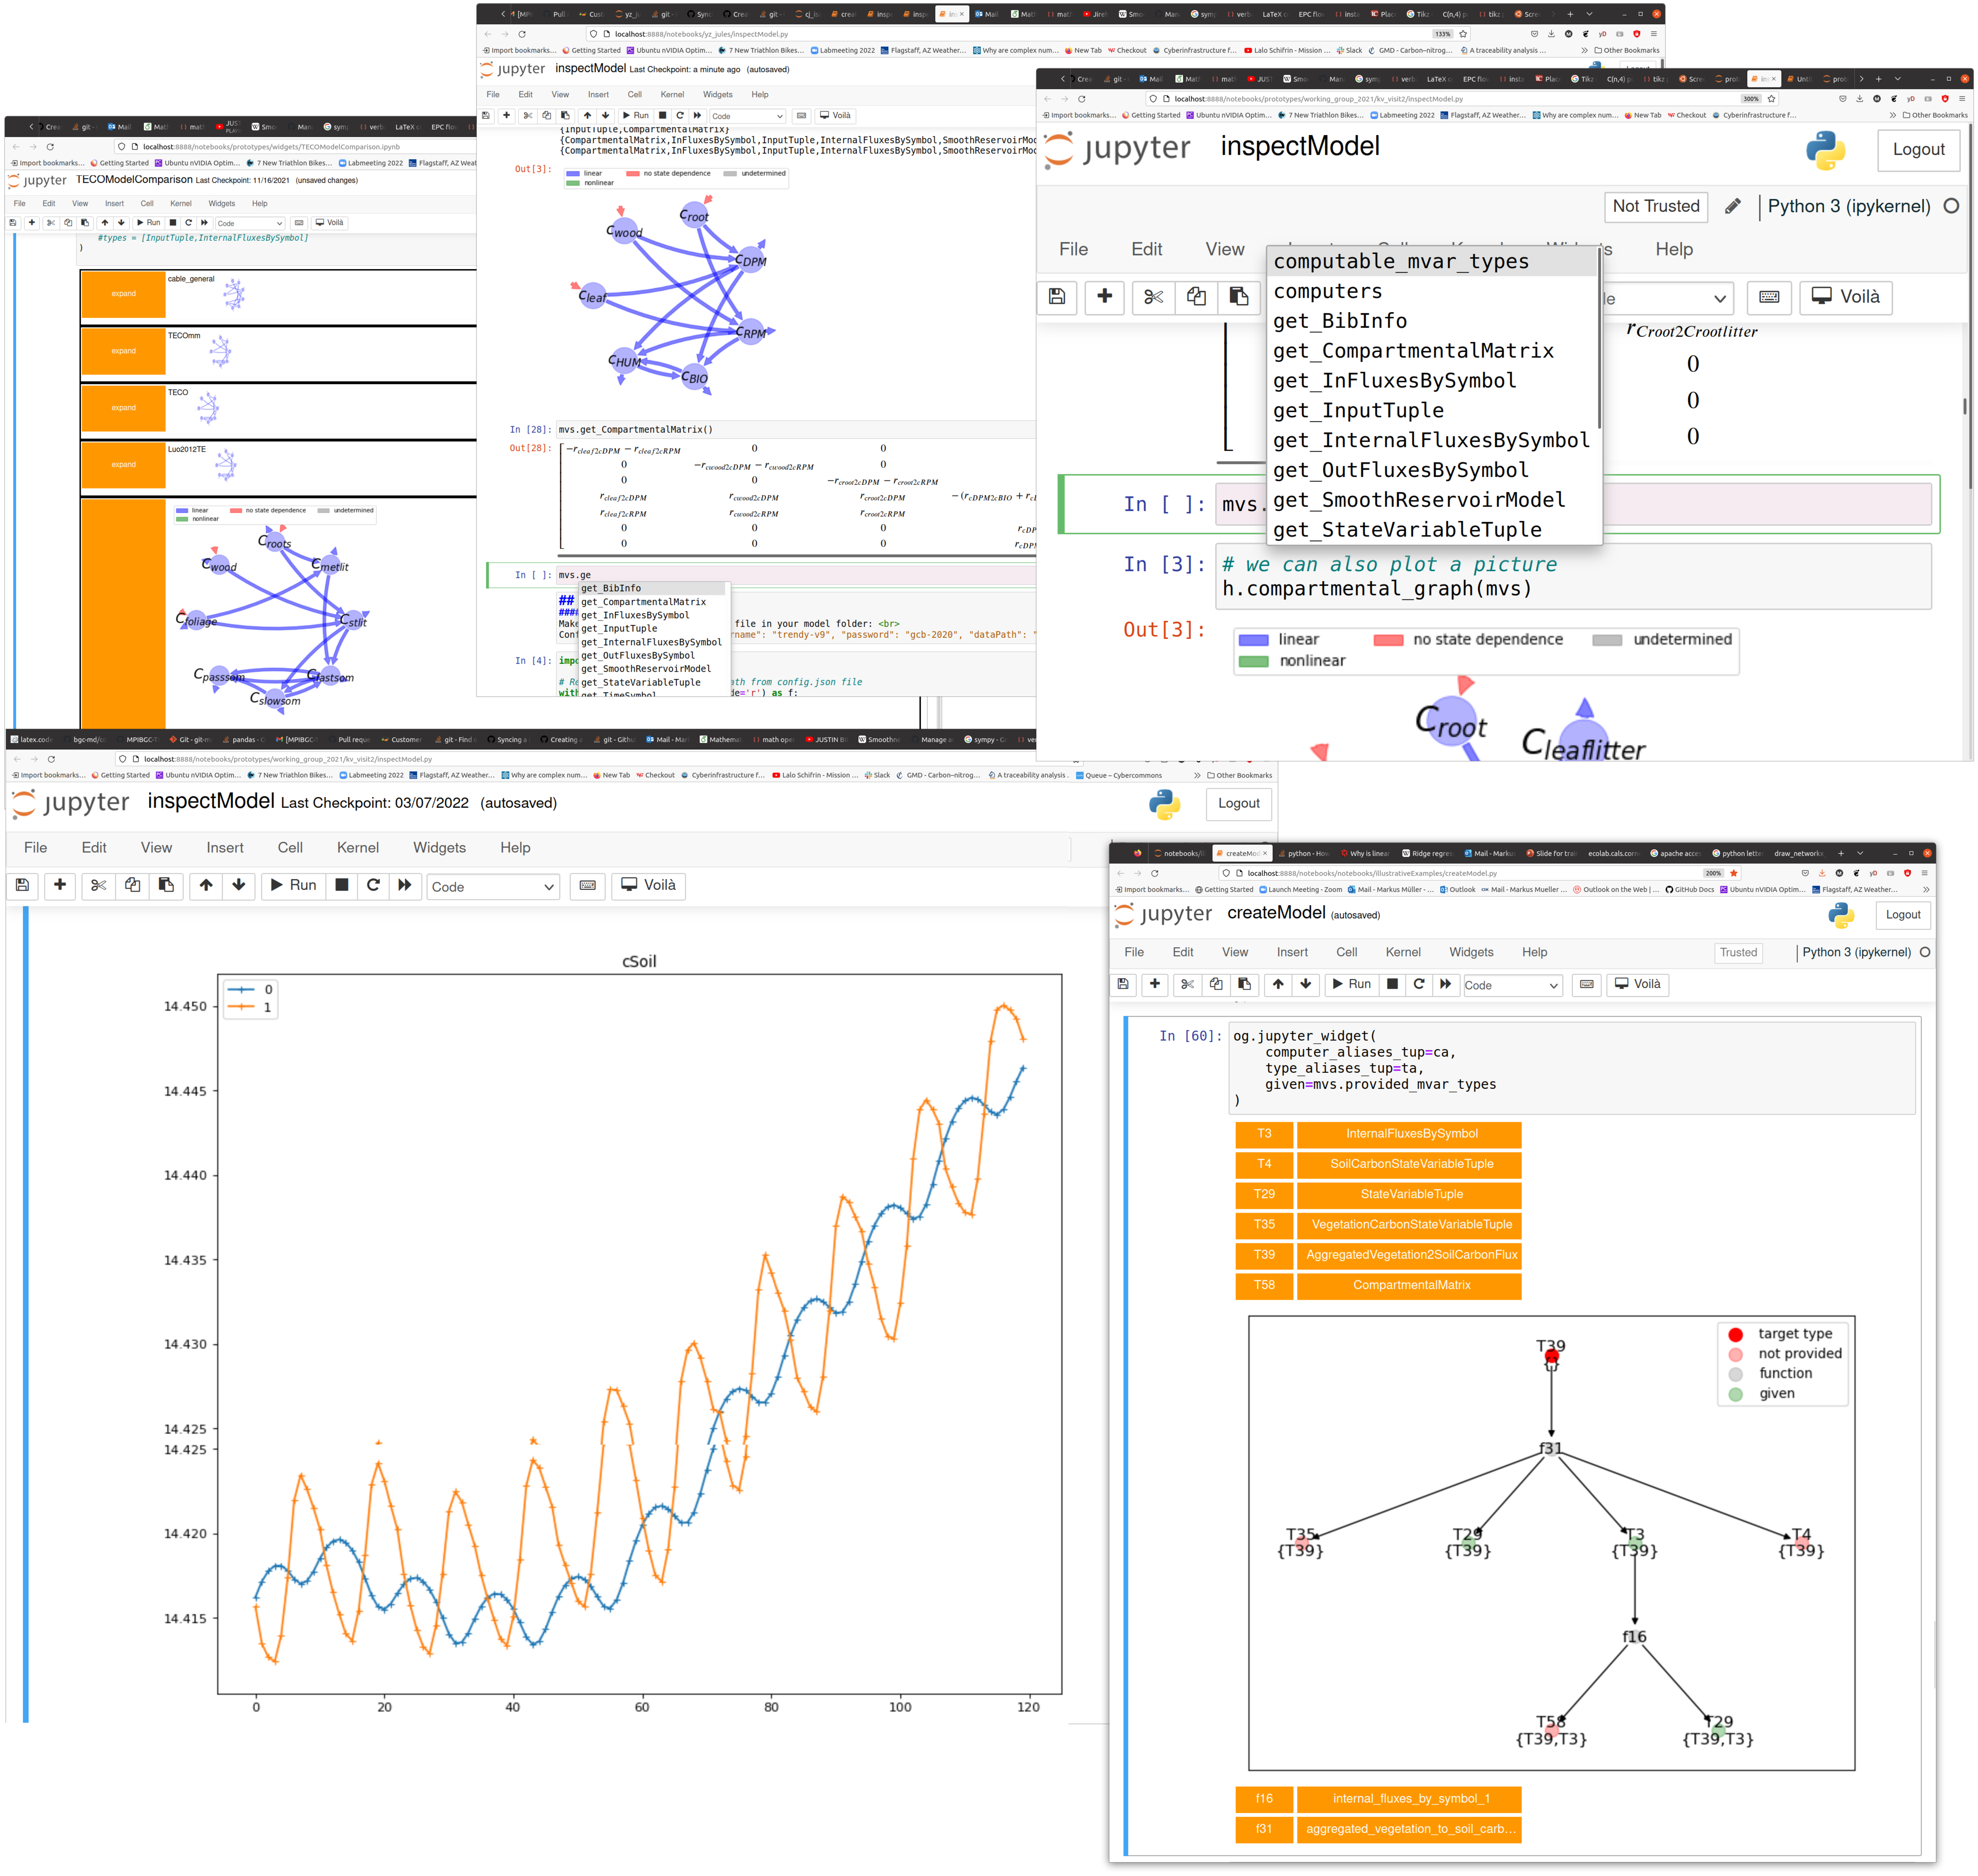
\includegraphics[width=\columnwidth]{TabScreenCombined.pdf}
  \caption{
      Figure description, top row, left to right: Interactive jupiter widget
      with a table of models (orange buttons can be clicked to expand or
      collape a more detailed view of the particular model), Model inspection
      with pool connection graph, which can be derived from the symbolic
      description along other symbolic properties as flux equations and the
      compartmental matrix, Zoom into IPython/Jupyter UI, showing methods
      automatically added by the computability graph library.  \\ Bottom row:
      Data assimilation with an automatically created numeric model (from
      symbolic description), Computability graph for a desired diagnostic
      (aggregated Flux from the vegetation to soil part, showing that the
      additionally needed information to compute the desired result)
  }
\end{figure}

\subsection{Installation, documentation and demonstrations}
The three packages are managed under version control in GitHub, and are publicly available for their evaluation, use, and further modification. They can be obtained using standard procedures for cloning and fetching Git repositories. 

The three packages can be installed following the instructions provided for the installation of \texttt{bgc\_md2}, which depends on \LAPM and \CompartmentalSystems, and therefore its installation script installs all packages at once. 
To install the packages, users must create a Python virtual environment using Conda and use the install script provided, which will take care that all dependencies required are properly installed. 
After installation, we strongly recommend users to run all test stored in the folder `tests'. If they run successfully, then all the functionality of the three packages is readily accesible. 

Detailed instructions of the installation procedure can be found in the `README.md' file of the \texttt{bgc\_md2} repository. 

We use docstrings to document modules, functions, classes and methods. These docstrings are snippets of human readable text included with the source code of the package, and are processed by Sphynx, a documentation generator for python code.  The formatted documentation is served by GitHub and it's automatically updated when changes to the documentation are pushed to the master branch of the repositories. 

In addition to this documentation, we provide Jupyter notebooks for each package, with demonstrations of specific aspects of the available functionality.
Each package has a 'notebooks' folder where the Jupyter notebooks are stored. However, they are stored as source .py files and not in the original .ipynb format. 
The reason for this is that to maintain the notebooks under version control and avoid conflicts among different versions on different machines, we store the notebooks as regular python files. To convert these files to Jupyter notebooks, we recommend to use Jupytext, which does the translation with a simple `convert' command. 
\begin{figure}[t]
	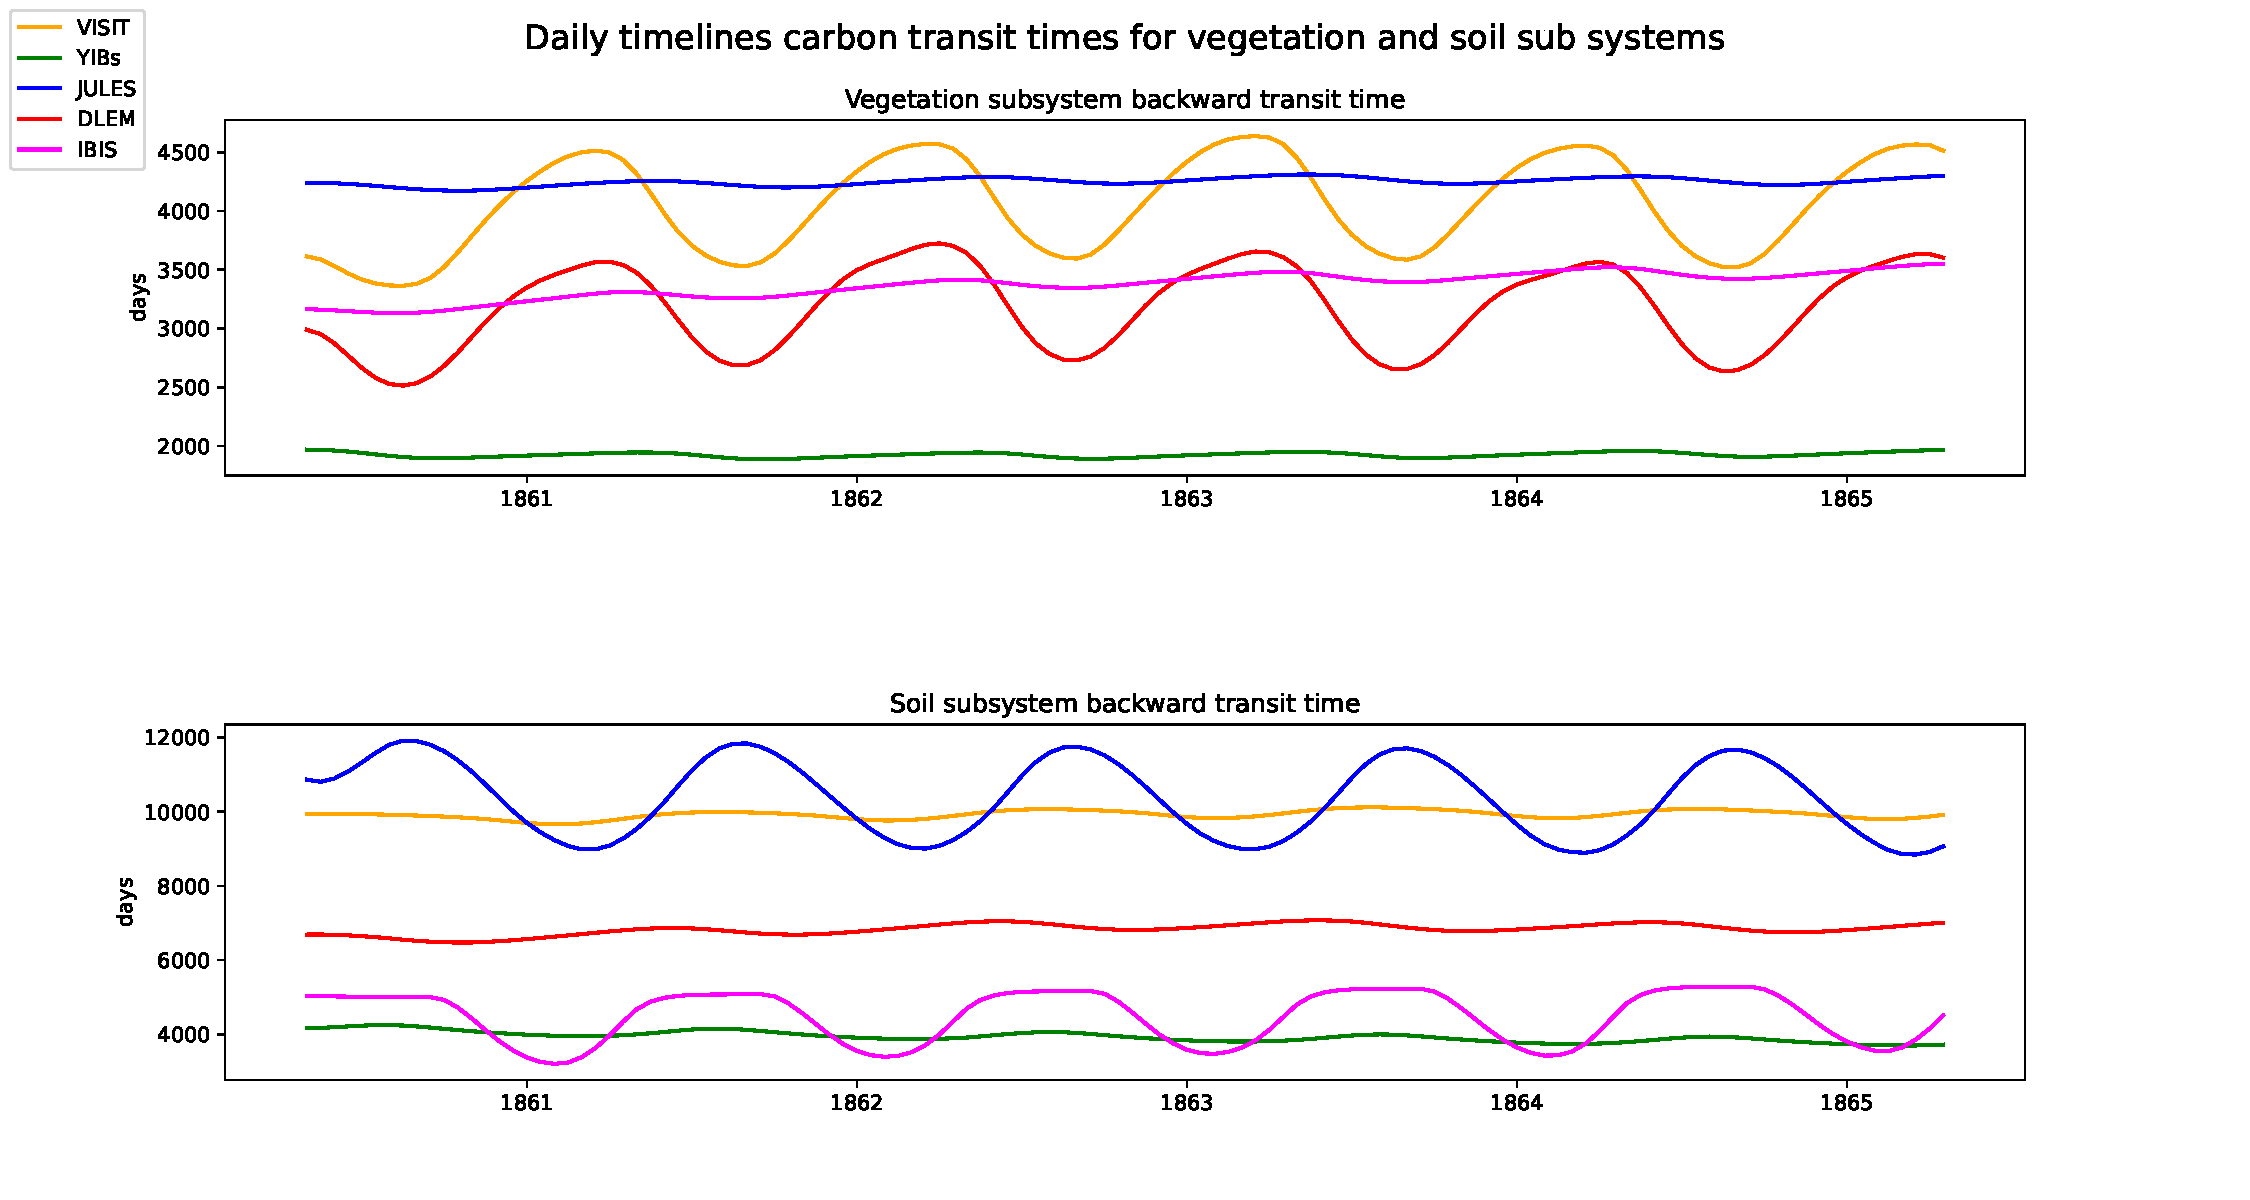
\includegraphics[width=\columnwidth]{test_veg_soil.pdf}
  \caption{
  Figure above: Comparing the (real = transient) backward transit time through 
  subsystems, accross different models. 
  }
\end{figure}  

\begin{figure}[t]
	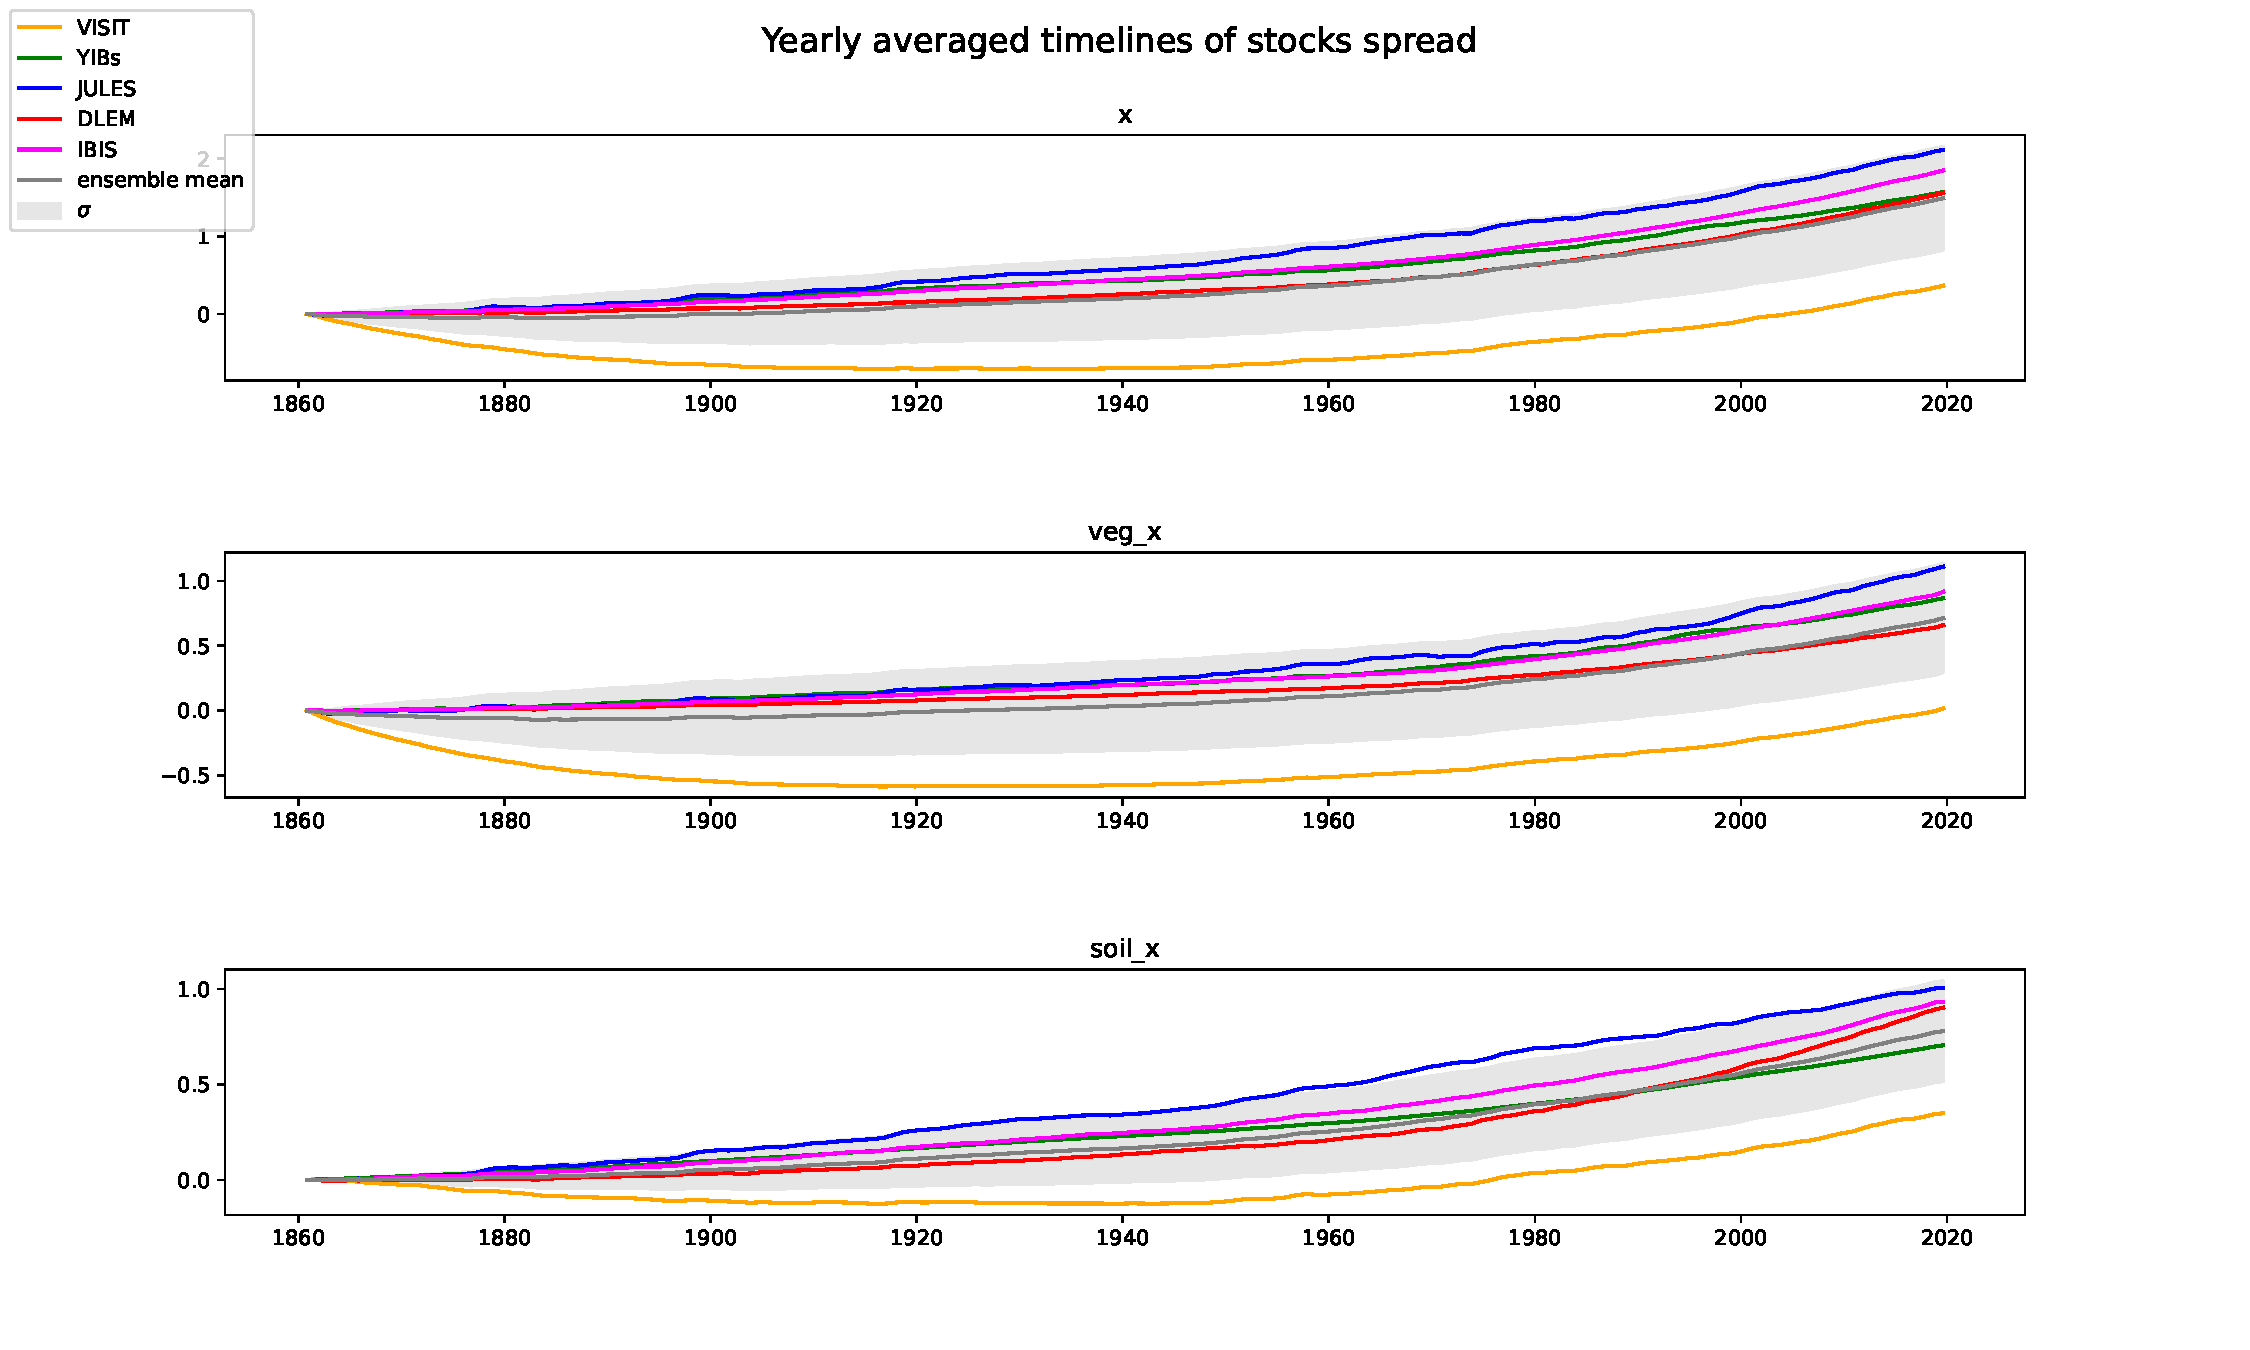
\includegraphics[width=\columnwidth]{test_stock_mean.pdf}
  \caption{
  Figure above: Total Carbon stock and subsystem stock development for different models.
  \texttt{bgc\_md} only needs to be told which pools belong to which subsystem.
  }
\end{figure}  

\section{\ComputabilityGraphs}
\begin{figure}[h]
  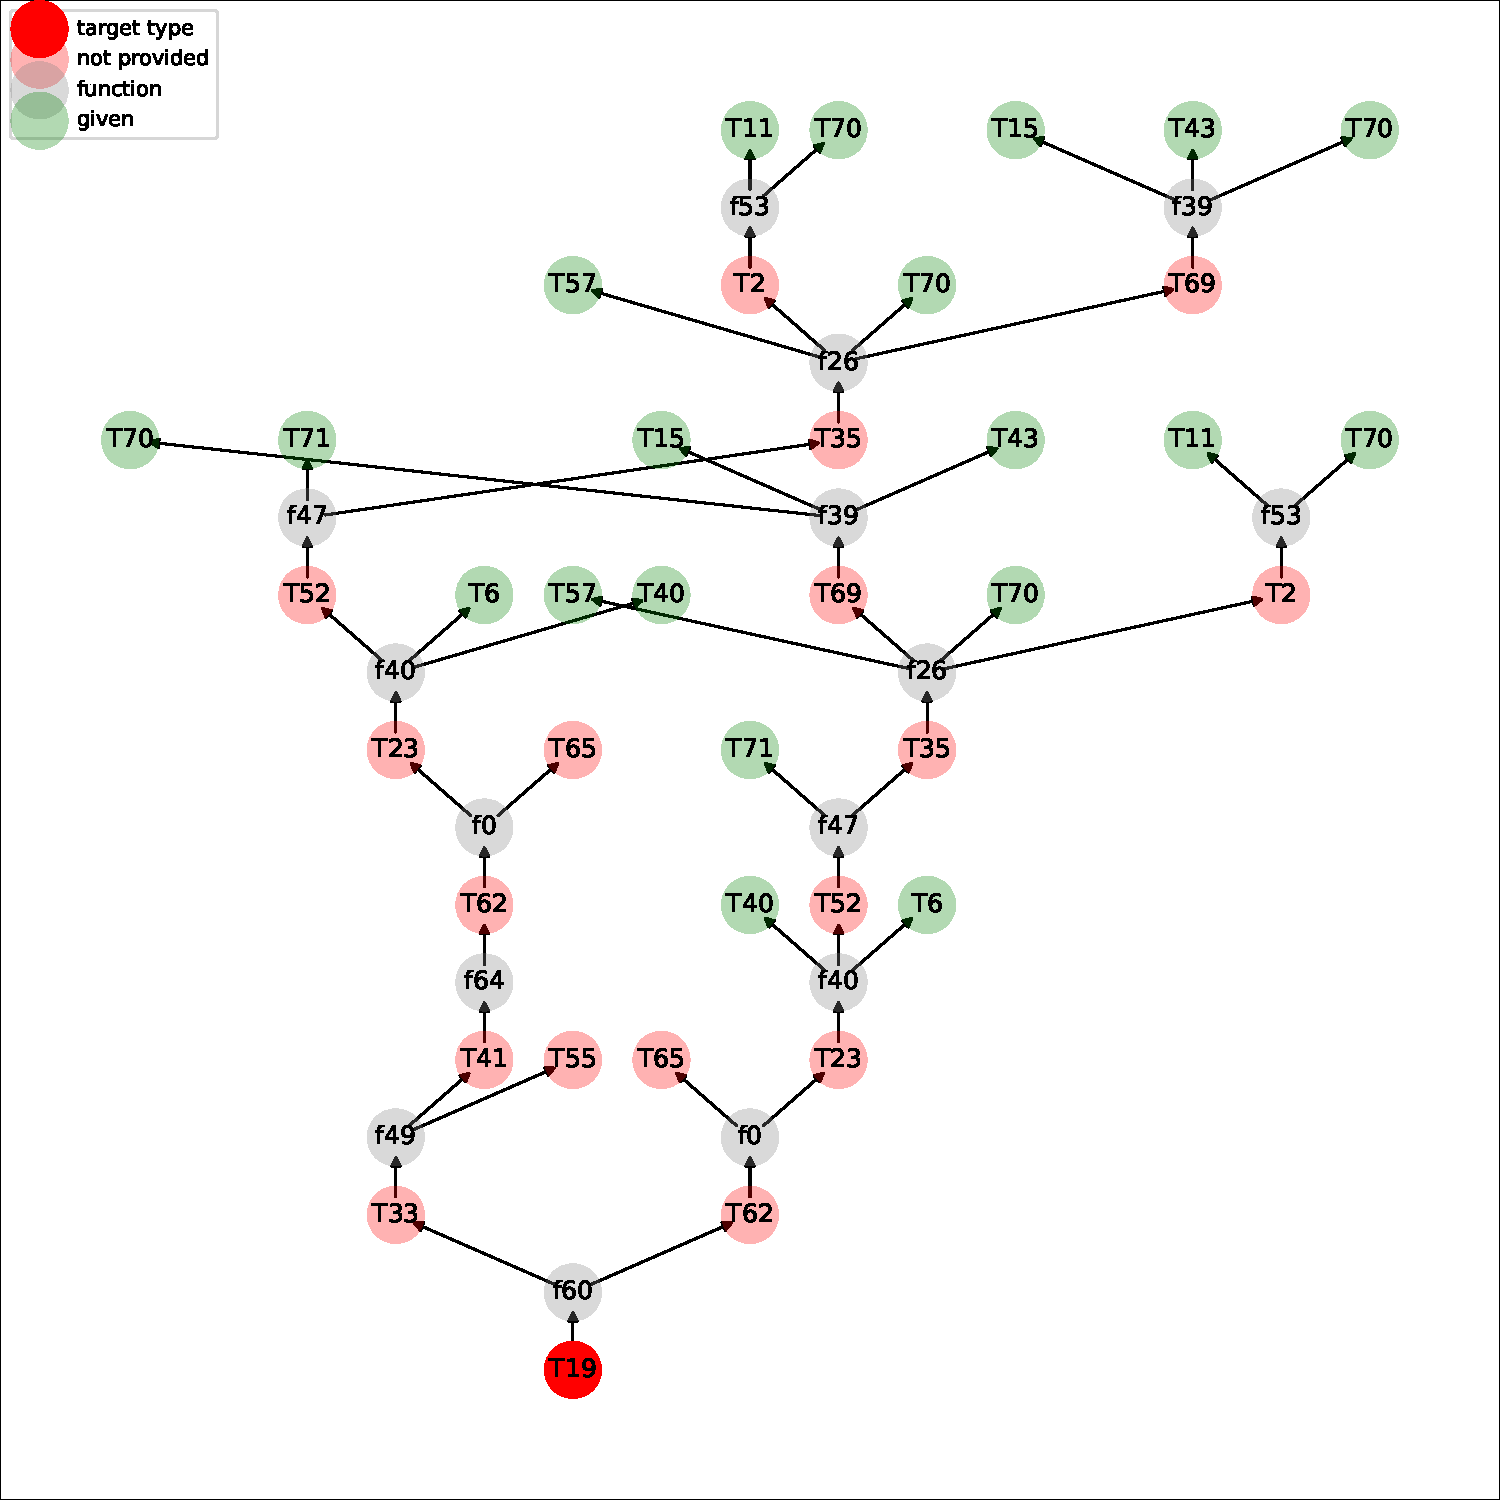
\includegraphics[width=\columnwidth]{bak_dep_graph.pdf}
  %\caption{
  %  Dependency graph for 
  %}
JAMES/TypeLegend.tex
\end{figure}  

\section{Illustrative example}
We provide an example notebook in
https://github.com/MPIBGC-TEE/bgc_md2/tree/master/notebooks/illustrative_example.
It shows the interplay of all three packages on the collection of predefined
models in \texttt{bgc\_md2} and ways to extend this collection by defining a new model
that can be compared with respect to diagnostic variables that are computed
using \LAPM and \CompartmentalSystems.  The best way to use the example is to
install the packages and explore the example interactively.
% This was an initial example I thought about showing how to compute ages and transit times along a trajectory for a nonlinear model

%We will show now an example on how to describe a simple nonlinear compartmental system to compute its age and transit time distribution both at equilibrium and along a particular solution trajectory. The model represents the dynamics of carbon in a soil, with one compartment representing the carbon substrate, and the other compartment representing the soil microbial biomass. We use the structure and parameterization described in \citet{Wang2014}. Due to the nonlinear relationship among the compartments, this model leads to strong oscillations for solution trajectories. 
%
%The model can be classified as a nonlinear autonomous model according to our definitions above, and can be written as
%\begin{equation}
%\left( \begin{matrix} \dot{C}_s \\ \dot{C}_b \end{matrix} \right) = 
%\left( \begin{matrix} F_{NPP} \\ 0 \end{matrix} \right) +
% \left( \begin{matrix}- \frac{C_{b} V_{s}}{C_{s} + K_{s}} &  \mu_{b} \\ \epsilon \frac{C_{b} V_{s}}{C_{s} + K_{s}}  & -  \mu_{b}\end{matrix}\right) \cdot
% \left( \begin{matrix} C_s \\ C_b \end{matrix} \right)
%\end{equation}

\section{Impact}


\section{Conclusions}


\bibliography{../../Bibliography/TEE-clean,../../Website/_bibliography/references,../../Website/_bibliography/theses,../../Theses/Holger/thesis/submitted_version/technical/bibliography}
\bibliographystyle{apalike}
\end{document}
